\chapter{Recorded numerical results}
\section{Six PID gain tables}
These values are read from the saved simulation summary. Order is
roll angle, roll rate, pitch angle, pitch rate, yaw rate, altitude. All
angular interfaces here are degree-based. The boot C defaults are the
$\lambda=1$ table; the selected video explicitly loads the $\lambda=1.3$
table through the host reset API. Neither table is authorized for physical flight.

\subsection{Baseline}
\begin{center}\begin{tabular}{lrrr}\toprule Controller & $K_p$ & $K_i$ & $K_d$\\\midrule
Roll angle & 3 & 0 & 0\\
Roll rate & 0.00118476874 & 0.00789845828 & 0\\
Pitch angle & 3 & 0 & 0\\
Pitch rate & 0.00118476874 & 0.00789845828 & 0\\
Yaw rate & 0.00767944893 & 0.0170654412 & 0\\
Altitude & 0.220500007 & 0.0900000036 & 0.174999997\\
\bottomrule\end{tabular}\end{center}

\subsection{Selected simulation}
\begin{center}\begin{tabular}{lrrr}\toprule Controller & $K_p$ & $K_i$ & $K_d$\\\midrule
Roll angle & 3 & 0 & 0\\
Roll rate & 0.00154019939 & 0.013348395 & 0\\
Pitch angle & 3 & 0 & 0\\
Pitch rate & 0.00154019939 & 0.013348395 & 0\\
Yaw rate & 0.00998328347 & 0.0288405959 & 0\\
Altitude & 0.372644991 & 0.197730005 & 0.227500007\\
\bottomrule\end{tabular}\end{center}
\section{Selection and route suite}
Every candidate is run on the same nominal seed 2350. A successful candidate
must avoid collision, end within 0.3 m of the 3D goal, and satisfy the navigator's
arrival conditions followed by one second dwell. Among successful nominal
candidates, the declared score is
\begin{equation}
J=t_f+20\,\mathrm{RMSE}_h+10\,\|p_f-p_g\|+\frac{2}{d_{\min}+0.01}.
\end{equation}
The coefficients are preference weights with implicit unit conversion; this
is not a dimensionless universal cost or a statistical estimator. Ranking
depends on clearance definition and weights. After including the complete
propeller envelope, the selected nominal case is nominal-1.3.
\begin{center}\small\begin{tabular}{lrrrrr}\toprule Case & $t_f$ [s] & Height RMS [m] & Final error [m] & Clearance [m] & Success\\\midrule
nominal-0.7 & 21.45 & 0.01057 & 0.13837 & 0.29061 & yes\\
nominal-1.0 & 21.50 & 0.01115 & 0.14035 & 0.29897 & yes\\
nominal-1.3 & 21.50 & 0.01199 & 0.14165 & 0.30058 & yes\\
heldout-heavy & 21.55 & 0.02968 & 0.14497 & 0.31306 & yes\\
heldout-weak-thrust & 21.60 & 0.03310 & 0.14106 & 0.29882 & yes\\
heldout-light & 20.35 & 0.03887 & 0.03652 & 0.27065 & yes\\
\bottomrule\end{tabular}\end{center}
Held-out scenarios do not change the selected gains: heavy mass is
$1.15m$ (seed 2351), weak thrust is $0.85T_{\max}$ (seed 2352), and light
mass/strong thrust is $0.85m$, $1.1T_{\max}$ (seed 2353). The controller hover
feed-forward is kept nominal, so the altitude integrator must compensate.
These three perturbations are not an exhaustive robustness region. Wind is a
one-second horizontal force of $(0.4,-0.3,0)$ N between 7 and 8 seconds. All
saved scenarios have zero motor-command saturation fraction. Initial motor
thrust is balanced for the physical test mass because these are airborne
route tests, not spool-up tests.
\begin{figure}[p]\centering
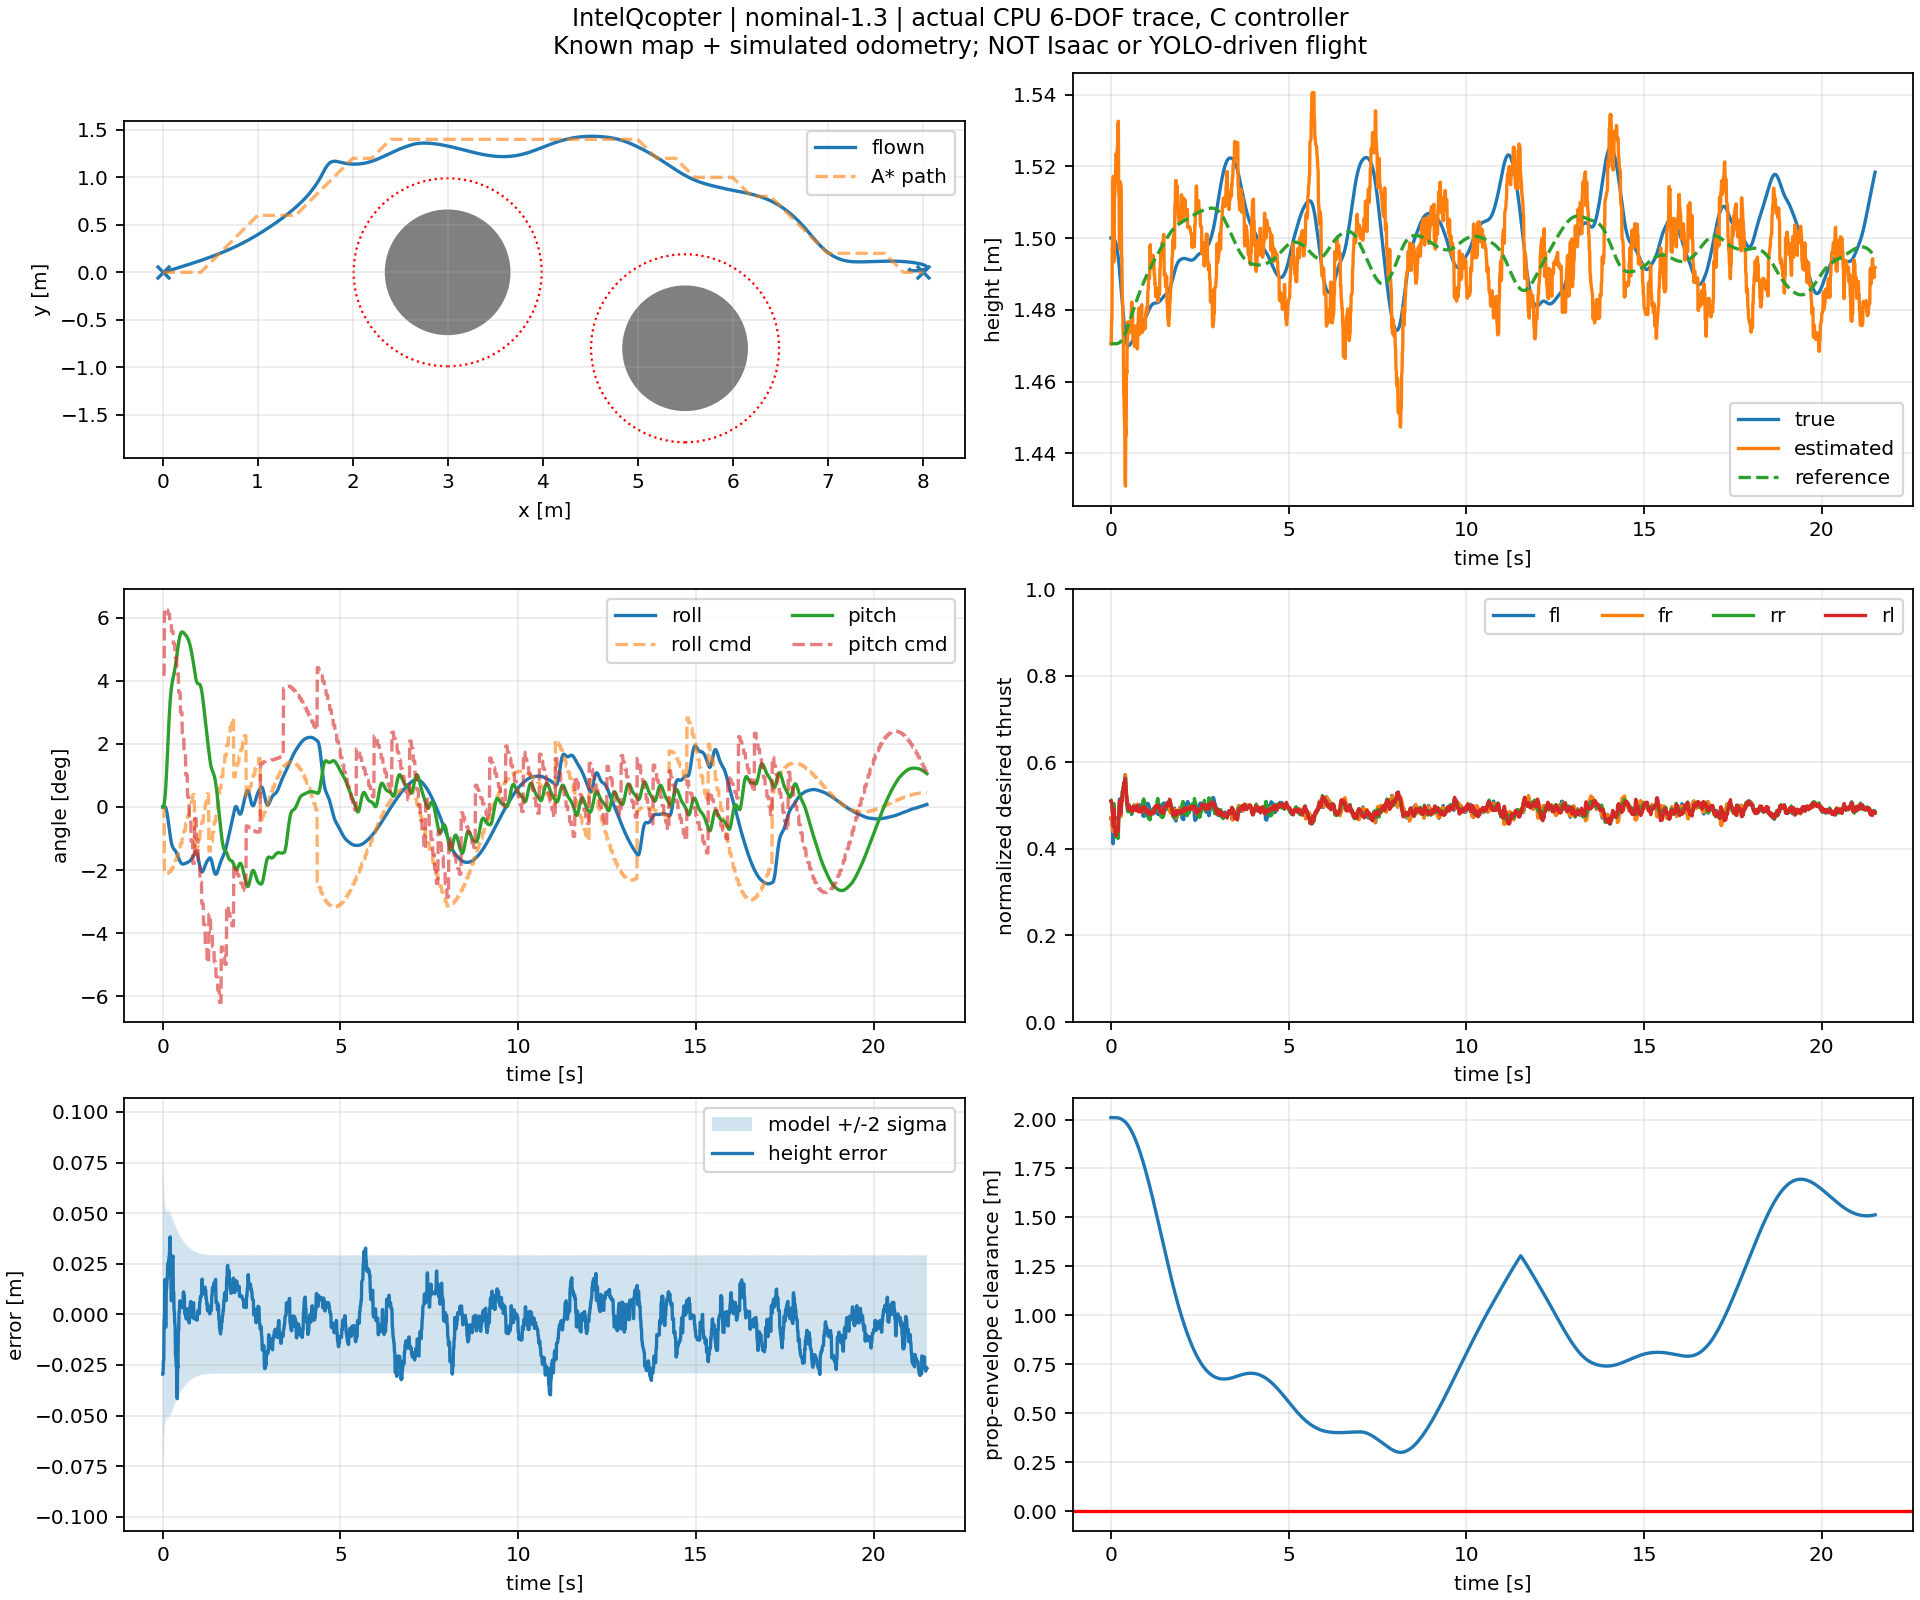
\includegraphics[width=\textwidth]{images/flight-results.png}
\caption{Original plots of saved CPU trace. Dashed circles include the propeller
envelope; the A* planner uses a larger planning inflation.}\end{figure}
\clearpage
\section{Kalman gains, standard deviation and distributions}
The final logged gains in the selected route are
\begin{align}
K_\theta&=0.00096639531, & K_b&=-0.000223559371\ \mathrm{s}^{-1},\\
K_h&=0.0834309161, & K_v&=0.181649998\ \mathrm{s}^{-1}.
\end{align}
These are end-of-run time-varying values, not preselected fixed constants. The selected route's roll and pitch estimation RMSEs are 0.75897 and 1.29857 degrees. Height error lies within its predicted two-sigma interval at 98.419\% of logged times. This is one correlated nonlinear trajectory and must not be interpreted as 500 independent statistical trials.
\begin{figure}[htbp]\centering
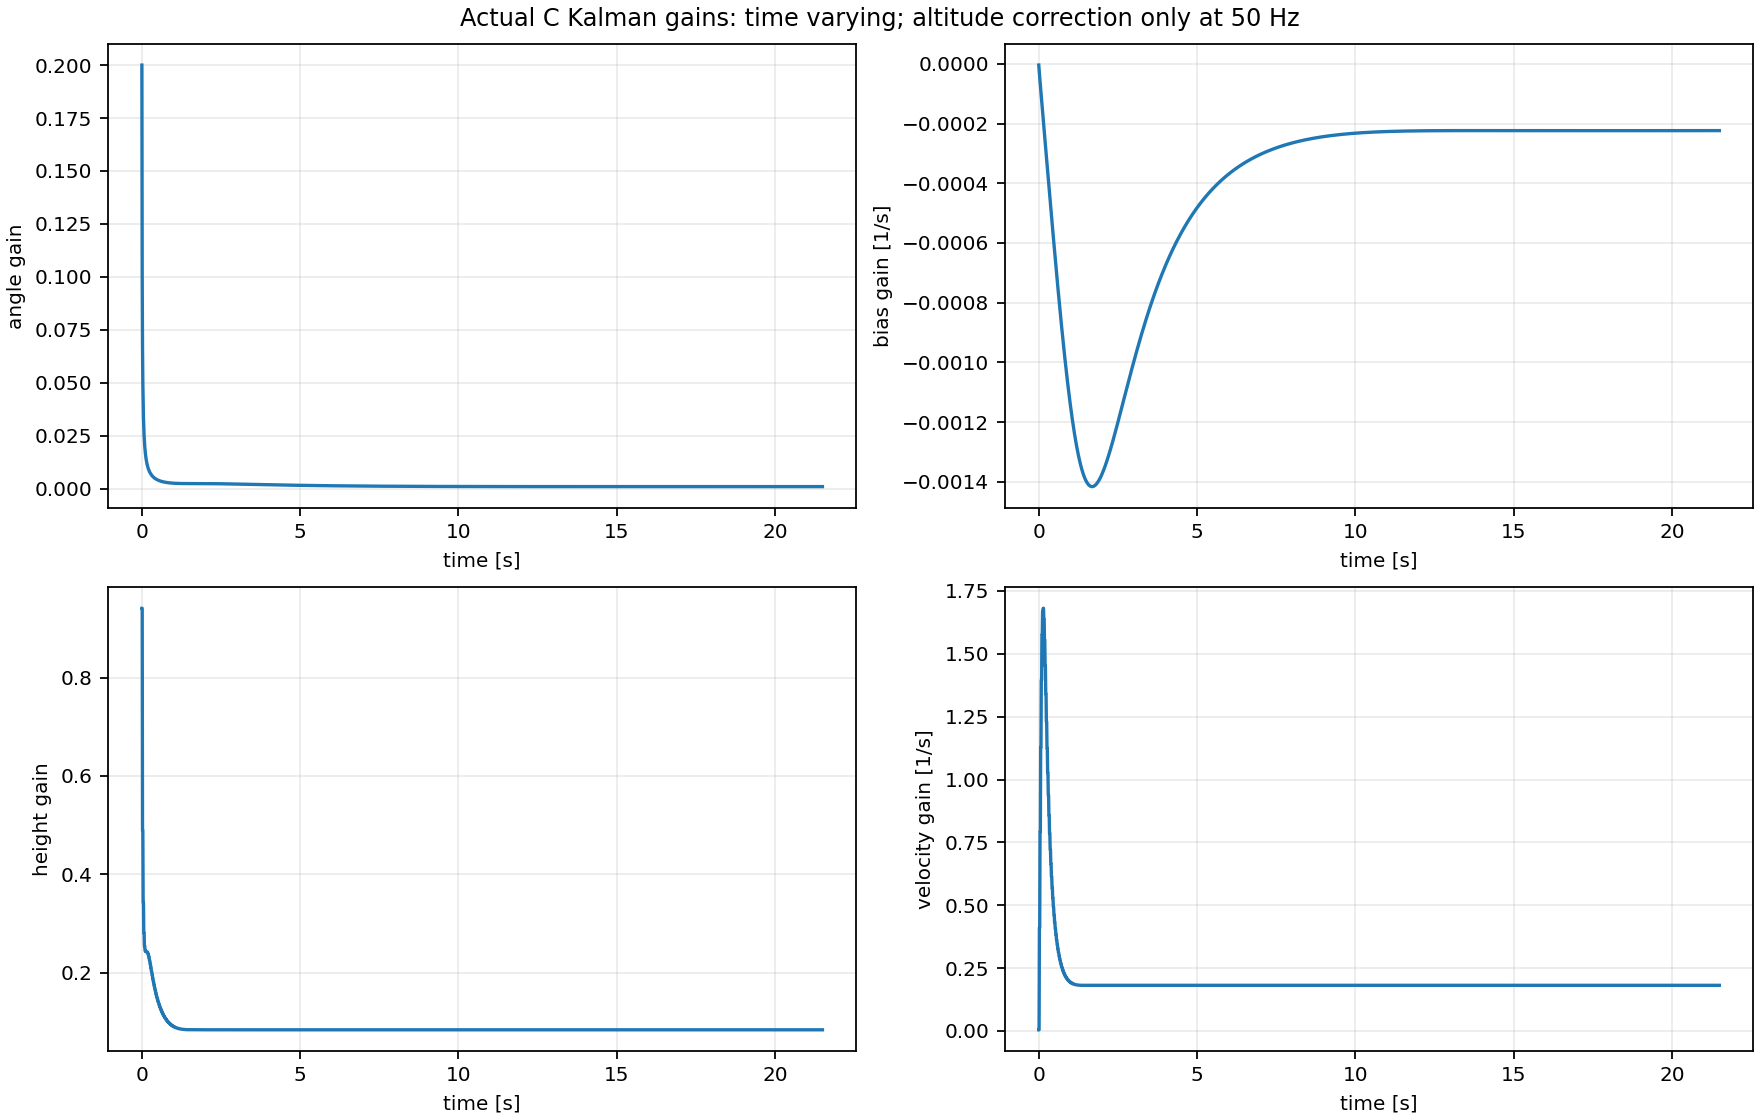
\includegraphics[width=\textwidth]{images/kalman-gains.png}
\caption{Actual gain evolution. Altitude gains are held between fresh barometer observations.}
\end{figure}
\subsection{Independent Monte Carlo experiments}
Both experiments call the production C estimator functions, with 500
synthetic independent trials of 2500 steps (5 seconds each). The angle test
uses seed 2350, prior angle sigma 1 degree, bias sigma 0.1 deg/s, gyro sample
sigma 0.2 deg/s, accelerometer-angle sigma 2 degrees, and bias random-walk
sigma 0.01 deg/s/$\sqrt{\mathrm{s}}$. It includes a prescribed eight-degree
ramp. The altitude test uses seed 2352, height prior sigma 0.2 m, speed prior
sigma $\sqrt{0.1}$ m/s, unobserved independent acceleration errors of sigma
1.5 m/s$^2$ per sample, and height observations of sigma 0.05 m at 50 Hz.
The altitude truth is propagated by exactly the held-acceleration stochastic
model used to derive $Q$. This tests statistical consistency under a matched
model, not realistic unknown airframe physics.
\begin{center}\begin{tabular}{lrrrr}\toprule
At final logged time & Mean error & Empirical std & Predicted std & $2\sigma$ coverage\\\midrule
Angle [deg] & -0.004526 & 0.078910 & 0.079017 & 95.00\%\\
Height [m] & -0.000296 & 0.013305 & 0.014442 & 96.80\%\\
\bottomrule\end{tabular}\end{center}
The angle generator samples bias Brownian motion at each endpoint while the
covariance includes the continuous interval integral; the difference is small
at 2 ms, but the test is not an exact continuous-noise sampler. Normalized
innovation checks and real sensor data are still needed before using these
intervals as engineering confidence claims.
\begin{figure}[htbp]\centering
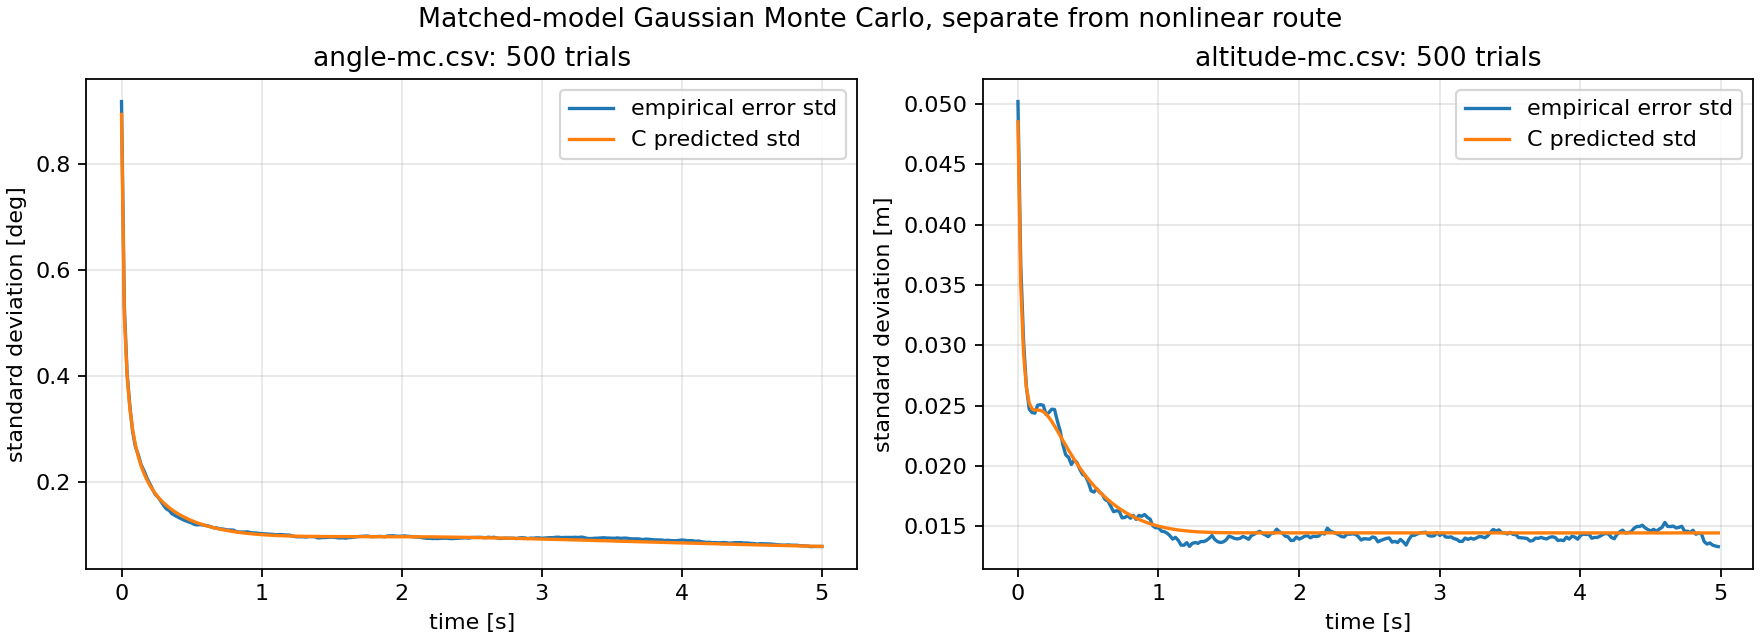
\includegraphics[width=\textwidth]{images/kalman-monte-carlo.png}
\caption{Empirical spread versus model-predicted spread; original C Monte Carlo data.}
\end{figure}
\clearpage
\section{Numerical refinement and algebra checks}
Host tests independently expand $FPF^{\mathsf T}$ and the Joseph correction,
check covariance symmetry and nonnegative determinants, and check positive
pitch increases rear thrust in FLU coordinates. Separate tests check rotation
orthogonality/determinant, matrix noncommutativity, nilpotence, stale navigation,
NaN navigation, out-of-map goals, occupied goals, blocked maps, depth-plane
back-projection and rejection of invalid depth. Linearized angular-rate and
altitude polynomials including the motor lag have strictly left-half-plane roots
for both baseline and selected gains. This does not include outer-loop,
estimator or sampled-data stability in that root test.

The selected case is repeated with unchanged 500 Hz sensing and control but
physical integration at 1 ms and 0.5 ms. The maximum aligned-time position
differences from the original 2 ms integration are:
\begin{center}\begin{tabular}{lrr}\toprule Physics interval & Max difference [m] & Route success\\\midrule
1.0 ms & 0.0017292 & yes\\
0.5 ms & 0.0025954 & yes\\
\bottomrule\end{tabular}\end{center}
The comparison bounds disagreement between these tested discretizations only.
It is not a rigorous global integration-error bound and does not measure
physical model error. Noise samples remain identical at the control interval.

\section{Executed ROS 2 communication test}
Two same-process Python adapter nodes exchanged 10,751 strictly sequenced request/response frames through Fast DDS UDPv4. Every received sensor/command envelope invoked the production C core; the result returned through DDS to the CPU plant. The best gain scale was used and the route succeeded. The median wall-clock round trip was 0.4693 ms, the 99th percentile 0.7514 ms, and the maximum 14.0538 ms.
The maximum can exceed the 2 ms control period; this is not a hard-real-time
500 Hz scheduling demonstration. The RP2350 is intended to own that local
loop; slow companion work must not block it. The two-node test is not an
independent-process or wireless benchmark and does not include a real UART.
The complete C++ ROS wrappers have been authored but not built on this PC.

\section{Executed YOLO and USD tests}
YOLO11n performed actual GPU inference on the official bus reference image: 5 detections. The warm measured inference phase reported 9.850 ms and the end-to-end warm call took 24.618 ms on this PC. One reference image is neither a perception benchmark nor a navigation safety test. Model and input SHA-256 hashes are saved in the JSON report.
The separately executed OpenCV DNN CPU test loaded the exported ONNX model, applied the C++ node's square-letterbox/raw-output/NMS contract, and produced 5 detections in an inference call of 97.894 ms. This exercised the portable inference engine through Python, not a running ROS C++ node. The raw output shape was $1\times84\times8400$ and the model hash is saved.
The ROS C++ YOLO source supports a raw YOLO11 ONNX model, letterboxing,
confidence thresholding, NMS and synchronized registered-depth annotation.
That C++ wrapper has not been compiled or executed here. The separate portable
USD scene is authored with positive assumed mass/inertia, four 9047 rotor
visuals, a conservative collision envelope, ground and obstacles. Its parser
and attributes are validated separately; it is not an executed Isaac scene.

\section{Files and reproducibility}
Project paths below are relative to the repository root, not shell commands
that install system software.
\begin{description}
\item[C firmware] \texttt{flight\_controller/flight\_controller.c}.
\item[Host checks] \texttt{tools/run\_flight\_controller\_tests.ps1}.
\item[Host libraries] \texttt{tools/build\_sitl.ps1}.
\item[CPU route] \texttt{sim/sitl/run.py}.
\item[Algebra/refinement] \texttt{sim/sitl/analysis\_tests.py}.
\item[DDS integration] \texttt{sim/ros2\_integration\_test.py} with bundled Isaac Python 3.12.
\item[Perception reference] \texttt{sim/yolo\_reference\_test.py}.
\item[USD authoring] \texttt{sim/isaac/build\_stage.py}.
\item[Graphs/video] \texttt{sim/sitl/visualize.py}.
\item[Data] \texttt{artifacts/simulation/2026-10-20/summary.json}, per-case CSVs,
Monte Carlo CSVs, \texttt{analysis-tests.json}, DDS and perception subdirectories.
\item[Original logs] \texttt{artifacts/test-runs/2026-10-20/}.
\item[Video] \texttt{artifacts/simulation/2026-10-20/best-flight-cpu.mp4}.
\end{description}
The video visualizes the selected saved trajectory at real-time playback speed
with live-progress graphs. It is not an Isaac recording, physical flight,
or a demonstration of YOLO-driven obstacle avoidance. Isaac remains blocked
by the recorded GPU startup failure on this workstation.
